% Este archivo es parte de la memoria del proyecto fin de carrera
% de Manuel López Urbina. Protegida bajo la licencia GFDL.
% Para más información, la licencia completa viene incluida en el
% fichero fdl-1.3.tex

% Copyright (C) 2018 Manuel López Urbina

\chapter[Estado del arte y herramientas utilizadas]{Estado del arte y herramientas utilizadas}
\chaptermark{Arte y tecnologías}
\label{chap:herramientas}


\section{ Estado del arte }

\subsection{Introducción}


Una de las mejores cosas de los robots es su capacidad para realizar trabajos que serían simplemente peligrosos para las personas. Los robots no solo pueden operar en entornos
donde los humanos no pueden, sino que también pueden enfrentar desafíos que son peligrosos.\\

Los robots pueden explorar en las profundidades del océano, investigar volcanes, zonas radiactivas, etc. En muchos casos, sin embargo, simplemente se hacen cargo de trabajos
que son tediosos y tienen un bajo margen de error como puede ser el caso de la soldadura, la cual es una parte muy importante de todo tipo de entornos de fabricación pesada.\\

En este tipo de trabajos, desafortunadamente, un instante de inatención puede significar un desastre para un soldador humano. No solo deben ser muy hábiles y precisos, sino que los errores pueden 
causar un gran desperdicio. Con los robots, se elimina el riesgo: el ruido, el calor intenso y los humos tóxicos no son un problema. Además, los robots pueden cambiar de un
proyecto a otro más rápido que las personas.\\

En el caso de la exploración de aguas profundas, incluso los buzos con equipo moderno y años de experiencia pueden sucumbir a diversos peligros, incluidos los depredadores del
mar y los efectos de las elevadas presiones. En la actualidad existen robots de exploración submarina capaces explorar y relaizar tareas 
a elevadas profundidades sin el peligro humano que estas acciones conllevarían.\\

Los robots han sido probados para una amplia gama de aplicaciones de respuesta a emergencias, incluyendo la extinción de incendios forestales, inundaciones y otras catástrofes
naturales.\\

Con el tiempo, los robots se especializarán y adaptarán cada vez mejor a situaciones que serían potencialmente letales para los humanos. Con una capacidad de maniobra y adaptación,
de lo que podemos concluir que los robots se han transformado en el compañero perfecto para cualquier tipo de misión de exploración o de rescate de alto riesgo.\\

Estas sistuaciones anteriormente descritas combinadas a que en la actualidad la robótica cada vez se encuentra más presente en nuestras vidas cotidianas hacen que cualquier usuario
pueda elaborar sus propios proyectos robóticos adaptables a cualquier entorno. Prueba de ello es que si realizamos cualquier búsqueda en internet podemos encontrar multitud 
de proyectos robóticos en la red. Existen excelentes portales como \url{http://blog.bricogeek.com/} por nombrar alguno de ellos, donde se
publican guías paso a paso de proyectos novedosos y originales para que cualquier usuario pueda hacerlos realidad.\\

Teniendo en cuenta éste contexto definido en actualidad, en la sección \ref{sec:referencias} se citan algunas de las referencias consultadas con la finalidad de contextualizar el proyecto 
en un ámbito más científico.\\

Por todo lo anterior nace SensorRS, un robot diseñado para operar en zonas peligrosas, el cual ha sido construido con medios asequibles para cualquier usuario pueda hacerlo realidad y 
personalizable y adaptable a situaciones concretas.\\

\subsection{ Referencias }
\label{sec:referencias}

Tras la realización de un sondeo entre numerosas bases de datos de artículos científicos existentes, indicar la existencia de artículos cuya temática guardan similitud con la problemática presentada
en cuanto a los requisitos y características del presente proyecto. Dichos artículos han sido tomados como punto de partida para el abordaje del problema y su estudio.\\

Existen numerosos artículos en los que se aborda el diseño y desarrollo y teleoperación de sistemas robóticos mediante la utilización de WebSockets y mediante la programación de microcontroladores. Por citar algunos de ellos como; \emph{Design and Development of a Robotic Teleoperation System using
Duplex WebSockets suitable for Variable Bandwidth Networks} \cite{article:1}, en el que se describe el desarrollo de un sistema teleoperable por WebSockets.\\
  
Otros estudios, en cambio, se centran más en analizar las diferentes situaciones de sobrecarga en la red, anchos de banda, cargas del sistema, etcétera, con la finalidad de someter a pruebas de estrés
los diferentes protocolos implicados. Como por ejemplo: \emph{Analysis of WebSockets as the New Age Protocol for Remote Robot Tele-operationt} \cite{article:2}.\\
  
Por otra parte, el artículo \emph{ Remote Monitoring System based on a Wi-Fi Controlled Car Using Raspberry Pi } \cite{article:3}, describe un sistema de monitorización construido sobre una placa 
Raspberry Pi de las mismas características que la empleada para el robot SensorRS.\\ 
  
  
También existen numerosos artículos donde detallándose el procedimiento para la construcción de proyectos robóticos con Arduino, como por ejemplo \emph{Design and Control of a Two-Wheel Self-Balancing Robot usin
g the Arduino Microcontroller Board} \cite{article-4} o proyectos que combinan el uso de una placa Raspberry Pi con una Arduino, como puede ser \emph{A Robotic-agent Platform For Embedding Software Agents usin Raspberry Pi and Arduino Boards} \cite{article:5}.\\
  
 
Es, por todo lo anterior, que en el presente proyecto se ha intentado dotar al sistema de una característica añadida. Permitir el seguimiento por parte parte del usuario que realiza las funciones de teleoperador. Además de enfocarlo
desde la perspectiva del entretenimiento y la enseñanza.\\


\section{Tecnologías software utilizadas}
\sectionmark{Tecnologías software}

A continuación se detallan las diferentes tecnologías/bibliotecas/lenguajes que se han empleado para la elaboración del proyecto y por qué se han escogido por encima de otras posibles soluciones.

\subsection{\LaTeX}

Web: \url{https://www.latex-project.org/}\\

\LaTeX \: es un lenguaje de marcado que sirve para la redacción de documentos científicos o técnicos. Con esta herramienta o lenguaje se ha desarrollado la memoria actual del proyecto de final de carrera.\\

Para el estudio de la herramienta y realización de consultas se han empleado sobre los recursos bibliográficos \cite{book:LaTeX} y \cite{website:6}.\\


\subsection{WebStorm}

\hspace*{2.25in}{
\includegraphics[scale=0.25]{imagenes/webstorm-logo.png}}

Web: \url{https://www.jetbrains.com/webstorm/}\\

WebStorm es un IDE de JavaScript ligero pero potente, perfectamente equipado para el desarrollo del lado del cliente (vehículo robótico) con Node.js. Para el desarrollo de la aplicación se optó por este IDE. \\

\subsection{Fritzing}

\hspace*{2.25in}{
\includegraphics[scale=0.5]{imagenes/fritzing-logo.png}}

Web: \url{https://http://fritzing.org/home//} \cite{website:1} \\

\\Fritzing es una iniciativa de hardware de código abierto que hace que los productos electrónicos sean accesibles como material creativo para cualquier persona.\\

Permitiendo la realización de diagramas, circuitos electrónicos y montajes, también sirve para hacer circuitos impresos PCB de manera profesional.

\subsection{Arduino IDE}

\hspace*{2.25in}{
\includegraphics[scale=0.5]{imagenes/arduino-logo.png}}

Web: \url{https://http://arduino.cc//} \cite{website:1} \\

El entorno de desarrollo ofrecido por Arduino resulta extremadamente sencillo de utilizar y de gran simpleza ya que el programa se escribe en la zona del sketch. Para compilarlo y
cargarlo a cualquier placa tan solo es necesario pulsar un botón.\\


\subsection{Github}

\hspace*{2.25in}{
\includegraphics[scale=0.25]{imagenes/github-logo.png}}

Web: \url{https://about.github.com/} \cite{website:2} \\
Repositorio: \url{https://github.com/lopi87/SensorRS}\\


GitHub es una forja (plataforma de desarrollo colaborativo) para alojar proyectos utilizando el sistema de control de versiones Git. Utiliza el framework Ruby on Rails por GitHub, Inc. (anteriormente conocida como Logical Awesome). Desde enero de 2010, GitHub opera bajo el nombre de GitHub, Inc. El código se almacena de forma pública, 
aunque también se puede hacer de forma privada, creando una cuenta de pago.\\

\subsection{Git}

\hspace*{2.1in}{
\includegraphics[scale=0.5]{imagenes/git-logo.png}}

Web: \url{https://git-scm.com/}\\

Git es un sistema open-source de control de versiones diseñado para manejar íntegramente las fases de desarrollo de proyectos, simples y complejos, con velocidad y eficiencia.\\

Para su estudio y afianzado de conocimientos, ya que este sistema de control de versiones me resultaba muy familiar incluso antes de comenzar con el desarrollo del presente proyecto, se ha empleado 
la referencia bibliográfica \cite{book:git}. La cual hace un recorrido por todas las posibilidades que brinda esta herramienta.\\


\subsection{Amazon Web Services (AWS) }

\begin{center}
\includegraphics[scale=0.25]{imagenes/aws_logo.png}\end{center}

Web: \url{https://aws.amazon.com/es}\\

Amazon Web Services (AWS) es una plataforma de servicios de nube que ofrece potencia de cómputo, almacenamiento de bases de datos, entrega de contenido y otra funcionalidad para ayudar a las empresas a escalar y crecer. Explore cómo millones de clientes aprovechan los productos y soluciones de la nube de AWS para crear aplicaciones sofisticadas y cada vez más flexibles, escalables y fiables.\\

\begin{sidewaysfigure}[H]
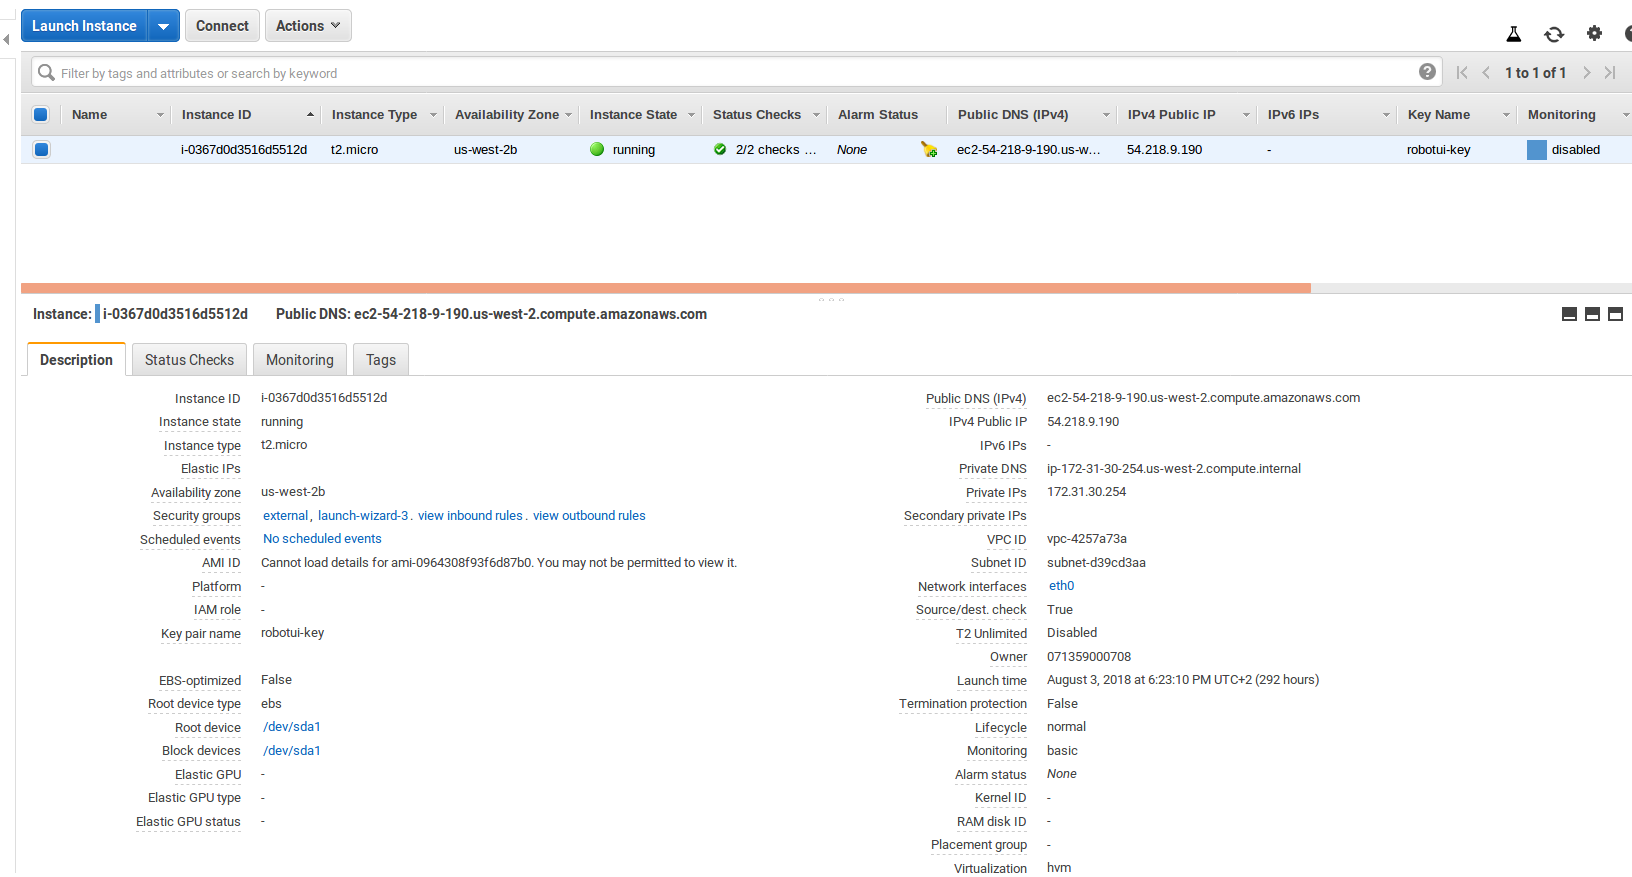
\includegraphics[scale=0.3]{imagenes/aws_instance.png}
\caption{Instancia RobotUI en AWS}
\end{sidewaysfigure}


\subsection{Node js}

\begin{center}

\includegraphics[scale=0.3]{imagenes/nodejs-logo.png}
\end{center}

Web: \url{https://nodejs.org/es/}\\
documentación: \url{https://nodejs.org/es/docs/}\cite{website:4}\\

Node.js es un entorno de ejecución para JavaScript construido con el motor de JavaScript V8 de Chrome. Node.js usa un modelo de operaciones E/S sin bloqueo y orientado a eventos, que lo hace liviano y eficiente. Incorpora un sistema de gestión de paquetes llamado, npm, es el ecosistema mas grande de librerías de código abierto en el mundo.\\

Node.js tiene una arquitectura basada en eventos capaz de E/S asíncronos. Estas opciones de diseño apuntan a optimizar el rendimiento y la escalabilidad en aplicaciones Web con muchas operaciones de entrada/salida, así como para aplicaciones Web en tiempo real (por ejemplo, programas de comunicación en tiempo real y juegos de navegador), lo que lo hacen ideal para este proyecto.\\

Destacar la importancia de la referencia bibliográfica \cite{book:javascript} para el estudio de tanto Node.js como JavaScript y que han servido de guía y consulta en la elaboración del presente proyecto. 
Sin olvidar la documentación oficial de Node.js \cite{website:4}.\\

\subsection{Npm}

\begin{center}

\includegraphics[scale=0.4]{imagenes/npm-logo.png}
\end{center}

Web: \url{https://www.npmjs.com/}\\

Npm es el gestor de paquetes por defecto para Node.js, un entorno de ejecución para JavaScript. Utilizado para la descarga de las librerías incorporadas al proyecto.


\subsection{SocketIO}

\begin{center}

\includegraphics[scale=0.3]{imagenes/socketio-logo.png}
\end{center}

Web: \url{https://socket.io/}\\

Socket.IO es una biblioteca de JavaScript para aplicaciones web en tiempo real. Permite la comunicación bidireccional en tiempo real entre clientes web y servidores. Consta de dos partes: una biblioteca del lado del cliente
que se ejecuta en el navegador y una biblioteca del lado del servidor para Node.js. Ambos componentes tienen una API casi idéntica. Al igual que Node.js, es impulsado por eventos.

Socket.IO puede usarse simplemente como un wrapper para WebSocket aunque proporciona muchas más funciones, incluyendo la transmisión a múltiples sockets, almacenamiento de datos asociados a cada cliente y E/S asíncronas.


\subsection{ FFmpeg }


\begin{center}

\includegraphics[scale=0.75]{imagenes/Ffmpeg-logo.jpg}
\end{center}

Web: \url{https://ffmpeg.org/}\\

FFmpeg es una colección bibliotecas software libre que permiten grabar, convertir (transcodificar) y hacer streaming de audio y vídeo. Incluye libavcodec, una biblioteca de códecs. FFmpeg está desarrollado en GNU/Linux, pero puede ser compilado
en la mayoría de los sistemas operativos, incluyendo Windows.\\

FFmpeg es un programa bastante sencillo y de fácil utilización, orientado tanto a personas con conocimientos avanzados como usuarios inexpertos. \\

El proyecto FFmpeg está compuesto por:\\

\begin{itemize}
 \item ffmpeg: es una herramienta de línea de comandos para convertir audio o video de un formato a otro. También puede capturar y codificar en tiempo real desde DirectShow, una tarjeta de televisión u otro dispositivo compatible.
 \item ffserver: es un servidor de streaming multimedia de emisiones en directo que soporta HTTP (la compatibilidad con RTSP está en desarrollo). Todavía no está en fase estable, y de momento no está disponible para Windows.
 \item ffplay: es un reproductor multimedia basado en SDL y las bibliotecas FFmpeg.
 \item libavcodec: es una biblioteca que contiene todos los códecs de FFmpeg. Muchos de ellos fueron desarrollados desde cero para asegurar una mayor eficiencia y un código altamente reutilizable.
 \item libavformat: es una biblioteca que contiene los multiplexadores/demultiplexadores para los archivos contenedores multimedia.
 \item libavutil: es una biblioteca de apoyo que contiene todas las rutinas comunes en las diferentes partes de FFmpeg.
 \item libpostproc: es una biblioteca de funciones de postproceso de vídeo.
 \item libswscale: es la biblioteca de escalado de vídeo.
\end{itemize}

Para el desarrollo de SensorRS, concretamente para la transmisión de vídeo desde el robot desarrollado hacia el servidor (aplicación web), el módulo utilizado ha sido el de la herramienta de línea de comandos.


\subsection{Bootstrap}


\begin{center}

\includegraphics[scale=0.3]{imagenes/bootstrap-logo.jpg}
\end{center}

Web: \url{http://getbootstrap.com/}\\

Bootstrap es un framework o conjunto de herramientas de código abierto para diseño de sitios y aplicaciones web. Contiene plantillas de diseño con tipografía, formularios, botones, cuadros, menús de navegación y otros elementos de diseño basado en HTML y CSS, así como, extensiones de JavaScript opcionales adicionales.
Se ha utilizado en el presente proyecto para la maquetación de la aplicación. En el presente proyecto se ha aprovechado para actualizarlo a la verisón 4.1.3, la más reciente hasta la fecha.\\  

\subsection{JQuery}


\begin{center}

\includegraphics[scale=0.7]{imagenes/jquery-logo.png}
\end{center}

Web: \url{https://jquery.com/}\\

JQuery es una biblioteca de JavaScript rápida, pequeña y característica. Hace que las cosas como manipulación del código HTML, manejo de eventos, animación, y permite la realización de 
peticiones Ajax de manera mucho más simple gracias a API de fácil manejo, la cual funciona a través de una multitud de navegadores. Gracias a su combinación de versatilidad y extensibilidad jQuery
ha cambiado la forma en que millones de personas desarrollan con JavaScript.\\


\section{Tecnologías hardware y materiales utilizados}
\sectionmark{Tecnologías hardware}
\label{sec:tecnologias-hardware}

A continuación se detallan las diferentes tecnologías hardware que se han
empleado para la elaboración del vehículo robótico con la finalidad de servir de prototipo durante el desarrollo de la aplicación y a modo demostrativo de la misma. En los sucesivos puntos
se describen las características de cada una de ellas junto con el motivo de su elección.


\subsection{Raspberry Pi Model B}
\label{sec:raspberry}


\begin{center}

\includegraphics[scale=0.3]{imagenes/RaspberryPi-logo.png}
\end{center}

Web: \url{https://www.raspberrypi.org}\\

Raspberry Pi es un ordenador de tamaño reducido y de bajo coste desarrollado en Reino Unido por la Fundación Raspberry Pi, con el objetivo de estimular la enseñanza de ciencias de la computación
en las escuelas. Es ampliamente utilizado y de uso muy extendido por lo que ha sido el principal motivo de su elección, además de su bajo cote y versatilidad.\\

La Raspberry Pi 3 es la tercera generación de Raspberry Pi. Sus especificaciones son las siguientes:

\begin{itemize}
 \item Una CPU ARMv8 quad-core de 64 bits de 64 bits y 1.2 GHz.
 \item LAN inalámbrica 802.11n.
 \item Bluetooth 4.1.
 \item Bluetooth baja energía (BLE).
 \item 1 GB de RAM.
 \item 4 puertos USB.
 \item 40 conexiones GPIO.
 \item Puerto HDMI.
 \item Puerto Ethernet.
 \item Conector de audio combinado de 3,5 mm y vídeo compuesto.
 \item Interfaz de la cámara (CSI).
 \item Interfaz de pantalla (DSI).
 \item Ranura para tarjeta Micro SD.
 \item VideoCore IV núcleo de gráficos 3D. 
\end{itemize}


\begin{figure}[H]
  \begin{center}
    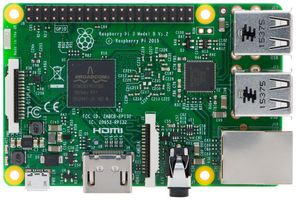
\includegraphics[scale=0.6]{imagenes/raspberry-pi.jpg}\\
    \caption{Imagen de una Raspberry Pi 3 Model B}
  \end{center}
\end{figure}


\subsection{ Arduino }

\begin{center}

\includegraphics[scale=0.6]{imagenes/arduino_logo.png}
\end{center}

Web: \url{https://www.arduino.cc/}\\

Arduino es una compañía open source y open hardware, así como un proyecto y comunidad internacional que diseña y manufactura placas de desarrollo de hardware para construir
dispositivos digitales y dispositivos interactivos que puedan sensar y controlar objetos del mundo real. Arduino se enfoca en acercar y facilitar el uso de la electrónica y 
programación de sistemas embebidos en proyectos multidisciplinarios. Los productos que vende la compañía son distribuidos como Hardware y Software Libre, bajo la Licencia Pública 
General Reducida de GNU (LGPL) o la Licencia Pública General de GNU (GPL),1​permitiendo la manufactura de las placas Arduino y distribución del software por cualquier individuo.
Las placas Arduino están disponibles comercialmente en forma de placas ensambladas o también en forma de kits hazlo tu mismo (DIY, por sus siglas en inglés de "Do It Yourself").\\

Los diseños de las placas Arduino usan diversos microcontroladores y microprocesadores. Generalmente el hardware consiste de un microcontrolador Atmel AVR, conectado bajo la 
configuración de "sistema mínimo" sobre una placa de circuito impreso a la que se le pueden conectar placas de expansión (shields) a través de la disposición de los puertos de 
entrada y salida presentes en la placa seleccionada. Las shields complementan la funcionalidad del modelo de placa empleada, agregando circuiteria, sensores y módulos de 
comunicación externos a la placa original. La mayoría de las placas Arduino pueden ser energizadas por un puerto USB o un puerto barrel Jack de 2.5mm. La mayoría de las placas 
Arduino pueden ser programadas a través del puerto Serial que incorporan haciendo uso del Bootloader que traen programado por defecto. El software de Arduino consiste de dos 
elementos: un entorno de desarrollo (IDE) (basado en el entorno de processing y en la estructura del lenguaje de programación Wiring), y en el cargador de arranque (bootloader,
por su traducción al inglés) que es ejecutado de forma automática dentro del microcontrolador en cuanto este se enciende. Las placas Arduino se programan mediante un computador, 
usando comunicación serial.\\


\begin{figure}[H]
  \begin{center}
    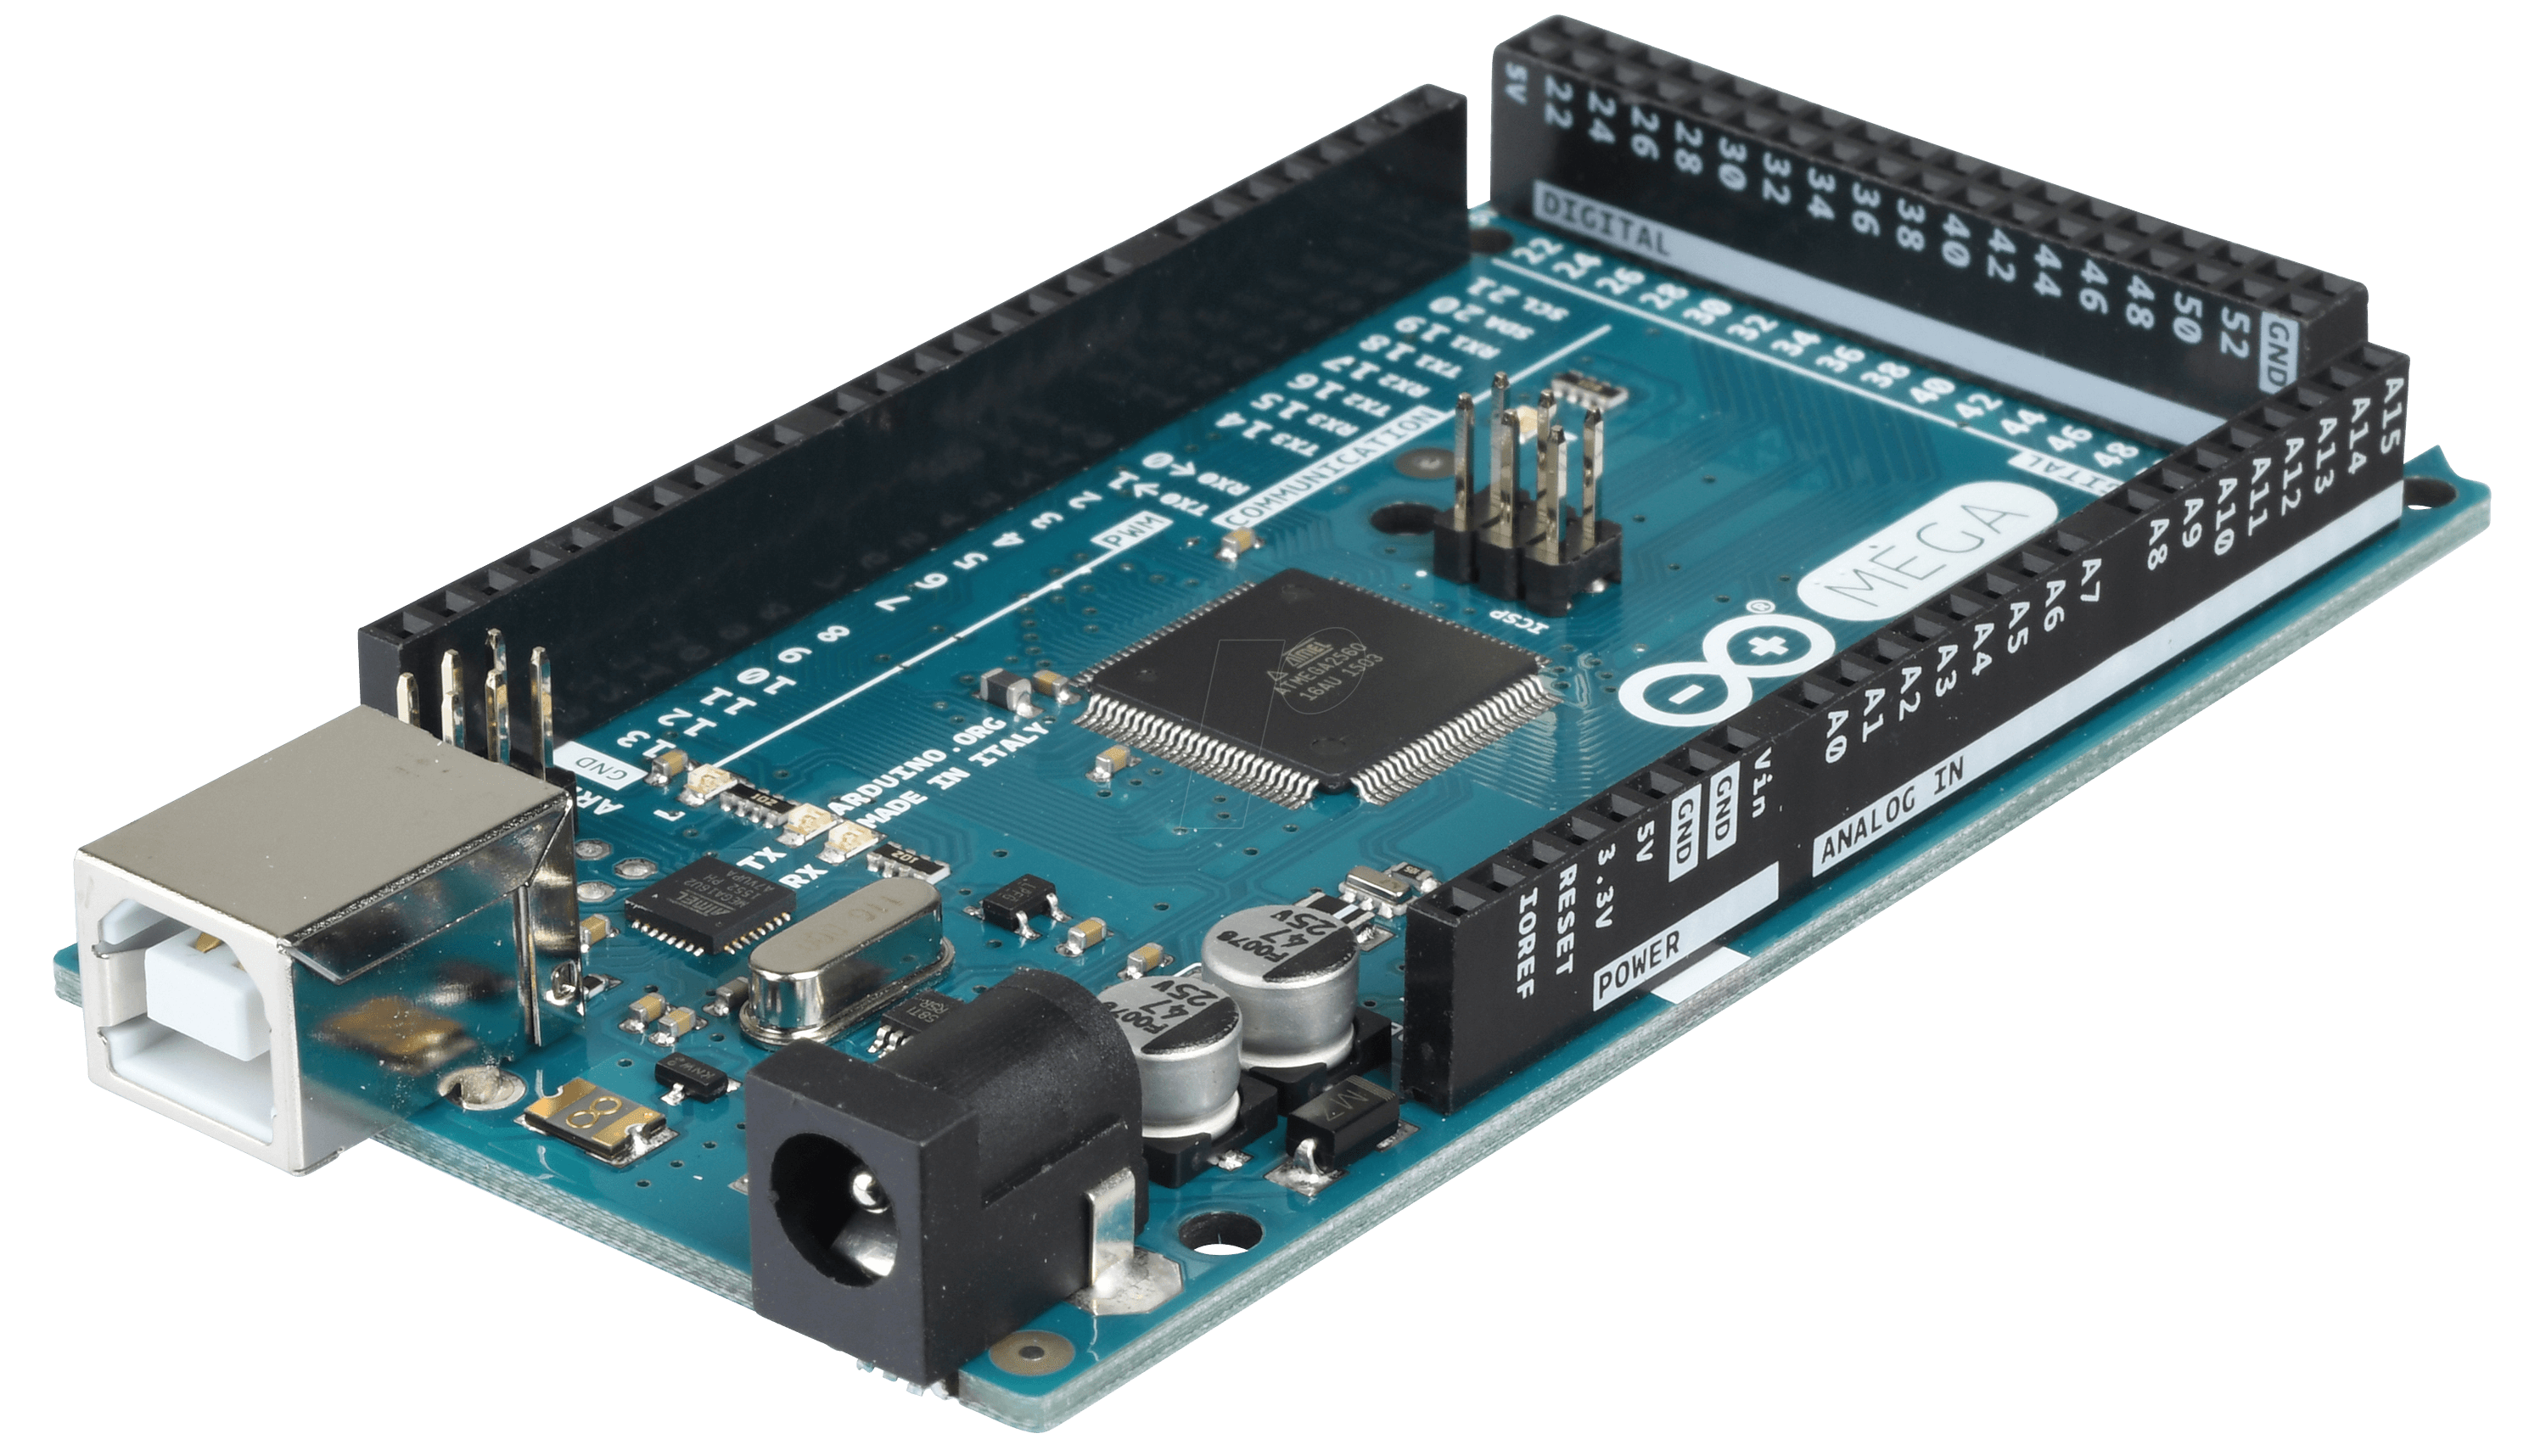
\includegraphics[scale=0.07]{imagenes/arduino_mega.png}\\
    \caption{Placa Arduino MEGA 2560}
  \end{center}
\end{figure}


Para el presente trabajo se ha utilizado la placa Arduino Mega, la cual es una tarjeta de desarrollo open-source construida con un microcontrolador modelo Atmega2560 que posee 
pines de entradas y salidas (E/S), analógicas y digitales. Esta tarjeta es programada en un entorno de desarrollo que implementa el lenguaje Processing/Wiring. Arduino puede
utilizarse en el desarrollo de objetos interactivos autónomos o puede comunicarse a un PC a través del puerto serial (conversión con USB) utilizando lenguajes como Flash,
Processing, MaxMSP, etc. Las posibilidades de realizar desarrollos basados en Arduino tienen como límite la imaginación.\\

El Arduino Mega tiene 54 pines de entradas/salidas digitales (14 de las cuales pueden ser utilizadas como salidas PWM), 16 entradas análogas, 4 UARTs (puertos serial por
hardware), cristal oscilador de 16MHz, conexión USB, jack de alimentación, conector ICSP y botón de reset.  Arduino Mega incorpora todo lo necesario para que el microcontrolador
trabaje; simplemente conéctalo a tu PC por medio de un cable USB o con una fuente de alimentación externa (9 hasta 12VDC). El Arduino Mega es compatible con la mayoría de los 
shields diseñados para Arduino Duemilanove, diecimila o UNO.

\begin{figure}[H]
  \begin{center}
    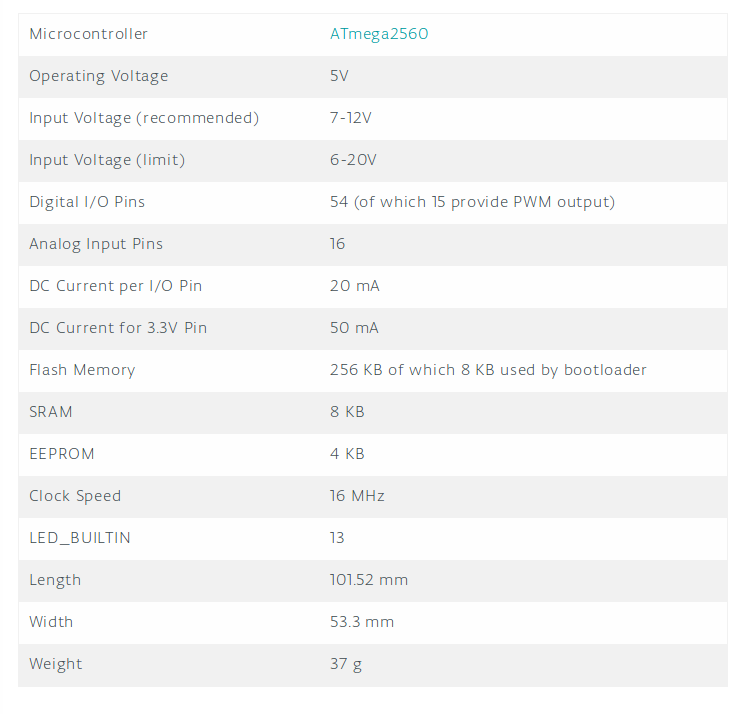
\includegraphics[scale=0.5]{imagenes/arduino_caracteristicas.png}\\
    \caption{Características Arduino MEGA 2560}
  \end{center}
\end{figure}


\subsection {Arduino sensor kit}

Se ha utilizado un pack de diversos sensores para arduino, los sensores utilizados quedarán descritos a mayor detalle en el capítulo referente a sensores \ref{chap:sensores}.

\begin{figure}[H]
  \begin{center}
    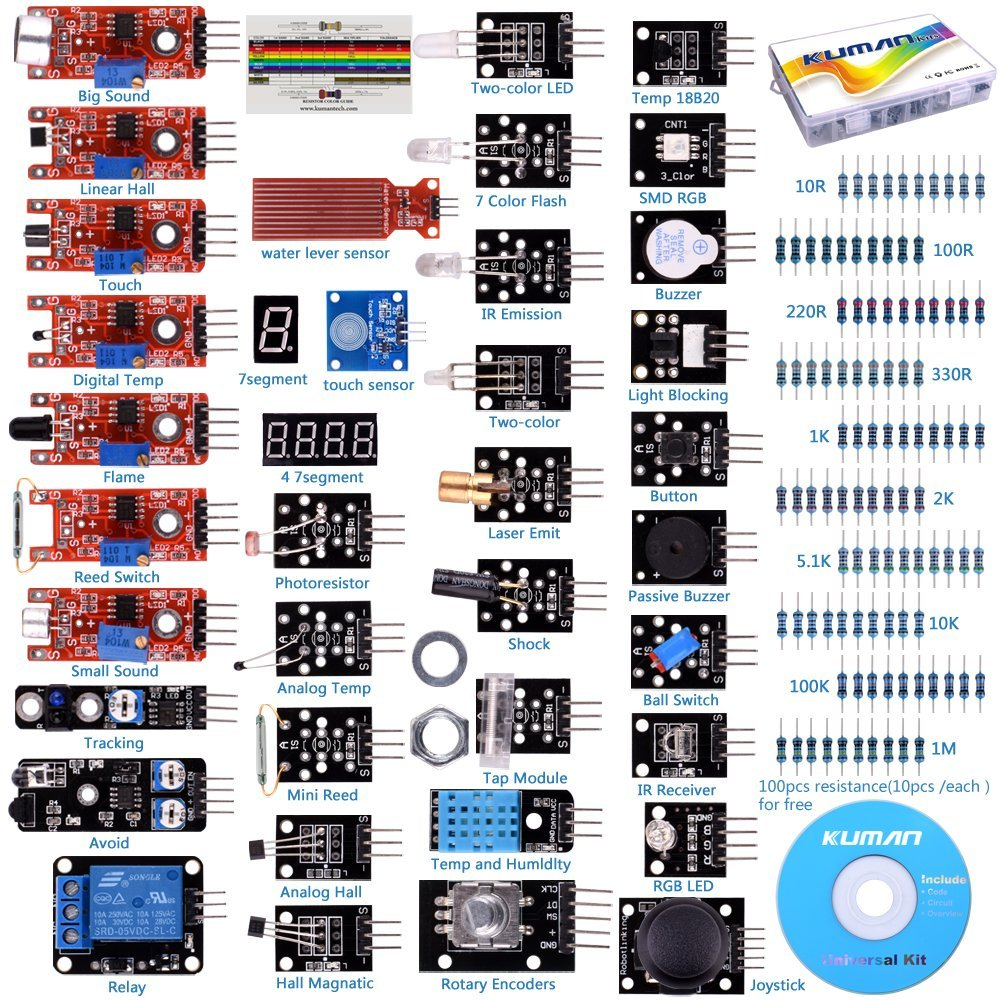
\includegraphics[scale=0.35]{imagenes/arduino_sensor_kit.jpg}\\
    \caption{Pack de sensores para Arduino}
  \end{center}
\end{figure}

\subsection{Controlador de motores doble puente H - L298N}


El módulo controlador de motores L298N H-bridge o puentes H, nos permite controlar la velocidad y la dirección de dos motores de corriente continua o un motor paso a paso de una forma muy sencilla,
gracias a los 2 los dos H-bridge que dispone.\\

Básicamente un puente-H o H-bridge es un componente formado por 4 transistores que nos permite invertir el sentido de la corriente, y de esta forma podemos 
invertir el sentido de giro del motor \footnote{Podrá acceder a información más detallada de la presente controladora en la sección correspondente al capítulo }.\\

El rango de tensiones en el que trabaja este módulo va desde 3V hasta 35V, y una intensidad de hasta 2A. A la hora de alimentarlo hay que tener en cuenta que la 
electrónica del módulo consume unos 3V, así que los motores reciben 3V menos que la tensión con la que alimentemos el módulo.\\

Además el L298N incluye un regulador de tensión que nos permite obtener del módulo una tensión de 5V, perfecta para alimentar nuestro Arduino. Eso sí, este regulador sólo 
funciona si alimentamos el módulo con una tensión máxima de 12V.\\

Es un módulo que se utiliza mucho en proyectos de robótica, por su facilidad de uso y su reducido precio, lo cual ha servido para que sea seleccionado para el presente proyecto.

\begin{figure}[H]
  \begin{center}
    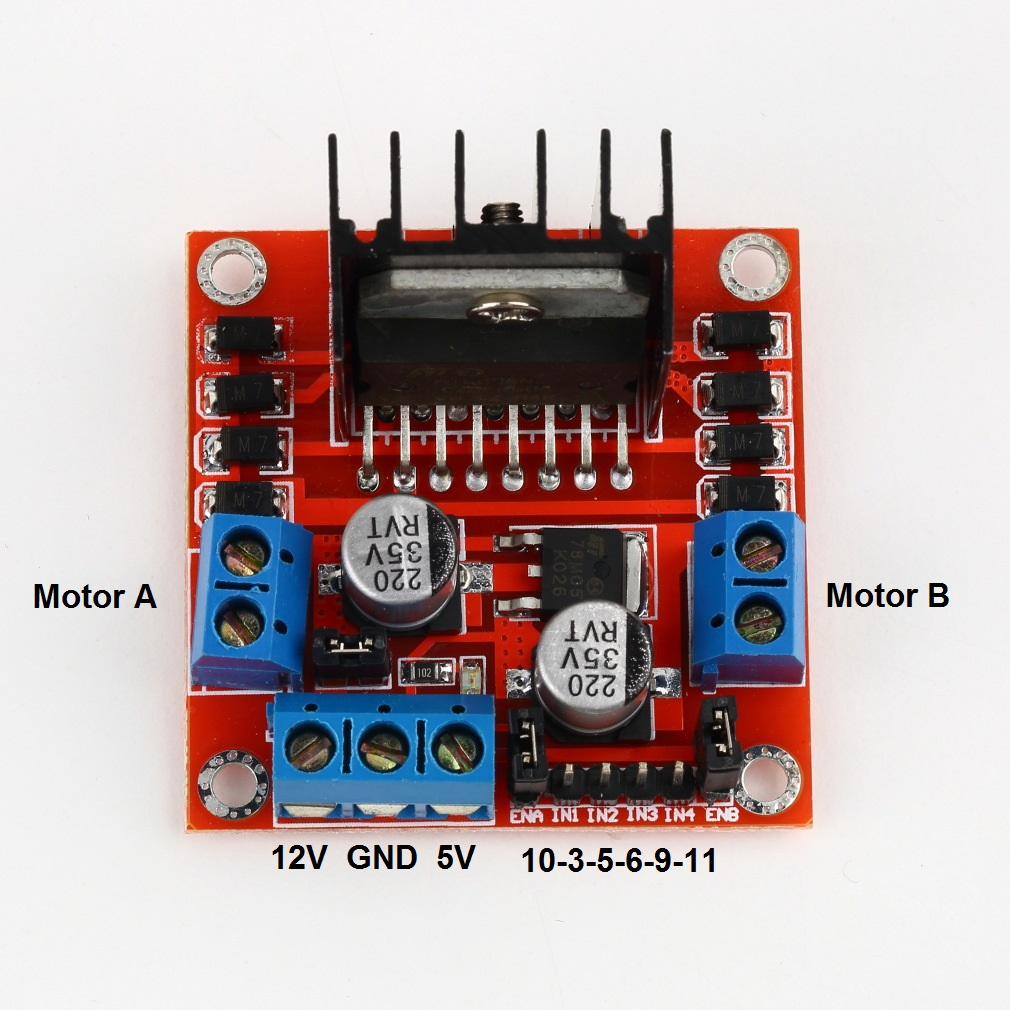
\includegraphics[scale=0.8]{imagenes/l298n.jpg}\\
    \caption{Imagen de la Controlador de motores doble puente H - L298N utilizada.}
  \end{center}
\end{figure}



\subsection{ Batería LiPo }

Para alimentar los motores y su controladora se ha empleado una batería LiPo de 2200mAh a 11,1V. Las batería de polímero de iones de litio, son pilas recargables (células de secundaria), compuestas generalmente 
de varias células secundarias idénticas en paralelo para aumentar la capacidad de la corriente de descarga. \\

Estas baterías son un tipo de batería recargable muy habitual en el mundo del modelismo, robótica, etc.  Nacen como una opción aceptable frente a la utilización
de combustibles siendo muy recomendables ya que ofrecen una prestaciones superiores a las NiCd y NiHmm.\\

\begin{figure}[H]
  \begin{center}
    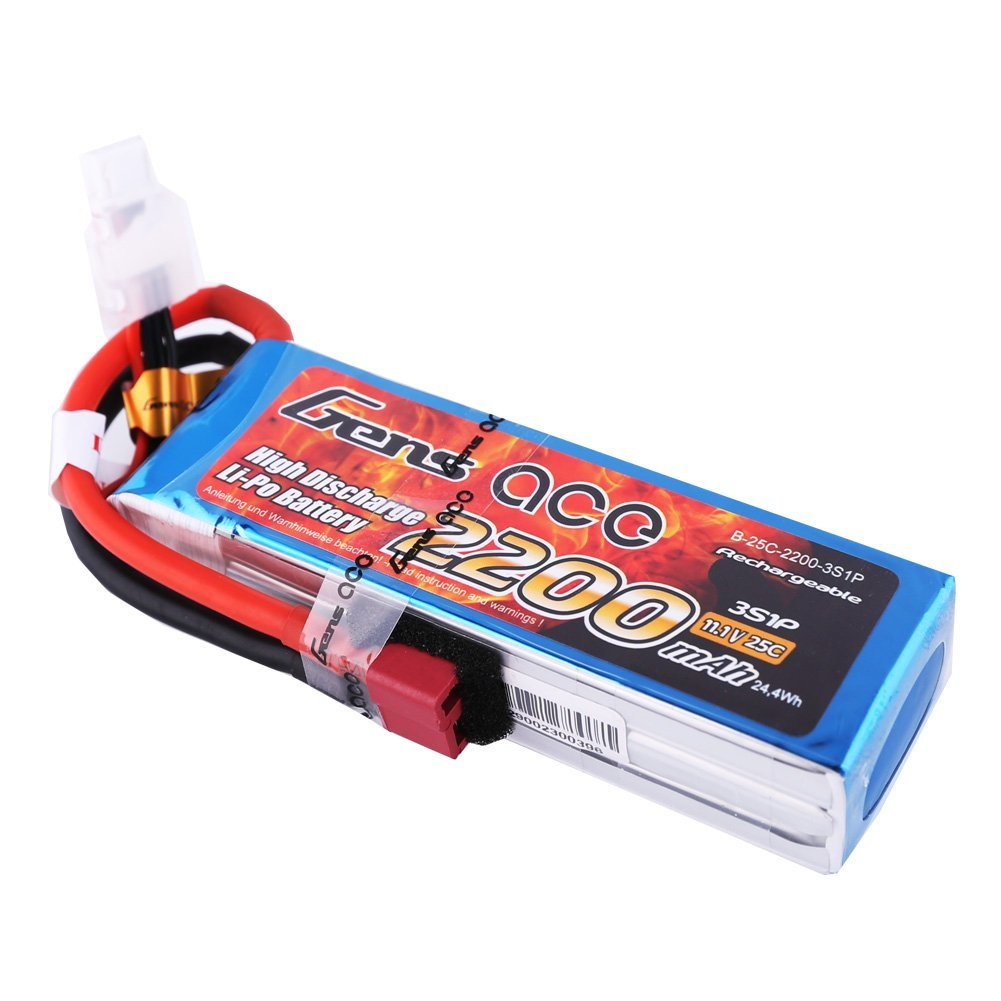
\includegraphics[scale=0.2]{imagenes/robot/bateria.jpg}\\
    \caption{Imagen de la batería LiPo utilizada.}
  \end{center}
\end{figure}

\subsection{ Alimentación USB/Protoboard }

Para alimentar la protoboard sin tener que modificar un cable USB, se ha decidido utilizar una pequeña tarjeta que se conecta en los carriles de tensión de la tarjeta Protoboard, y
proporciona los 5 V de entrada del USB (o de un conector Jack) a las líneas de alimentación de la protoboard. Además este dispositivo integra un interruptor, que permitirá activar y
desactivar los motores, y puede regular la tensión a 3,3 Voltios.\\

\begin{figure}[H]
  \begin{center}
    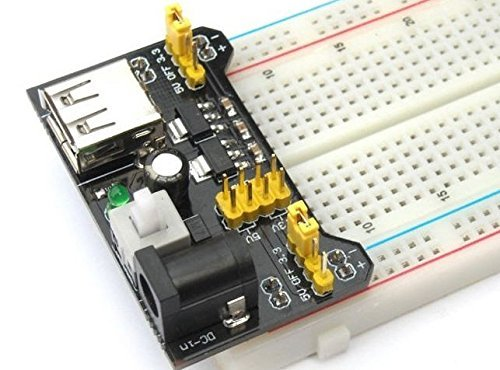
\includegraphics[scale=0.3]{imagenes/alimentador_usb_protoboard.jpg}
  \end{center}
  \caption{Adaptador de entrada USB a protoboard utilizado.}
  \label{figura:alimentador_placa_usb_protoboard}
\end{figure}


\subsection{ Tarjeta de expansión con batería de Litio para Raspberry Pi }
\label{componente:bateria-expansion}

Para la alimentación de la placa se ha optado por un módulo de potencia diseñado especialmente para la Raspberry Pi 3 Model B, permitiendo que la placa maestra trabaje sin conexión hasta 9 horas
de forma ininterrumpida.\\

Por otra parte, esta placa dispone de 2 puertos USB adicionales: uno suministra energía para la Raspberry Pi y el otro para una posible pantalla LCD, resultando interesante para otros proyectos.\\

Sus características principales son las siguientes:

\begin{enumerate}
 \item Capacidad de la batería: 3800mAH.
 \item Corriente de descarga máxima: 1.8A.
 \item Tensión de salida sin carga: 5.1V ± 0.1V.
 \item Corriente / voltaje de carga estándar: 1.0A / 5.0V.
 \item Tensión de corte de la carga completa de la batería de iones de litio: 4.18V - 4.2V.
\end{enumerate}


\begin{figure}[H]
  \begin{center}
    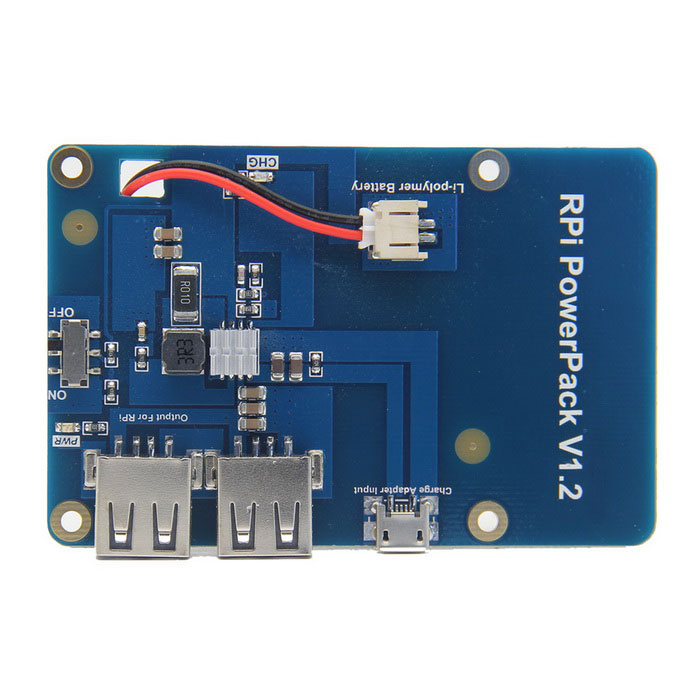
\includegraphics[scale=0.3]{imagenes/robot/modulo-alimentacion.jpg}\\
    \caption{Imagen de la tarjeta de expansión con batería de Litio utilizado.}
  \end{center}
\end{figure}

\subsection{ Cámara USB de alta definición }

Cámara USB para su conexión en la Raspberry para la emisión de imágenes. La cámara seleccionada dispone de las siguientes características:

\begin{itemize}
\item 2 megapíxeles de resolución.
\item Ángulo de visión de 170 grados.
\item Interfaz USB 2.0 de alta velocidad, refresco de 60 fps en resolución 1280X720, 30 fps en resolución 1920X1080.
\item Tamaño reducido y perfil delgado ideal para aplicaciones embebidas.
\end{itemize}

\begin{figure}[H]
  \begin{center}
    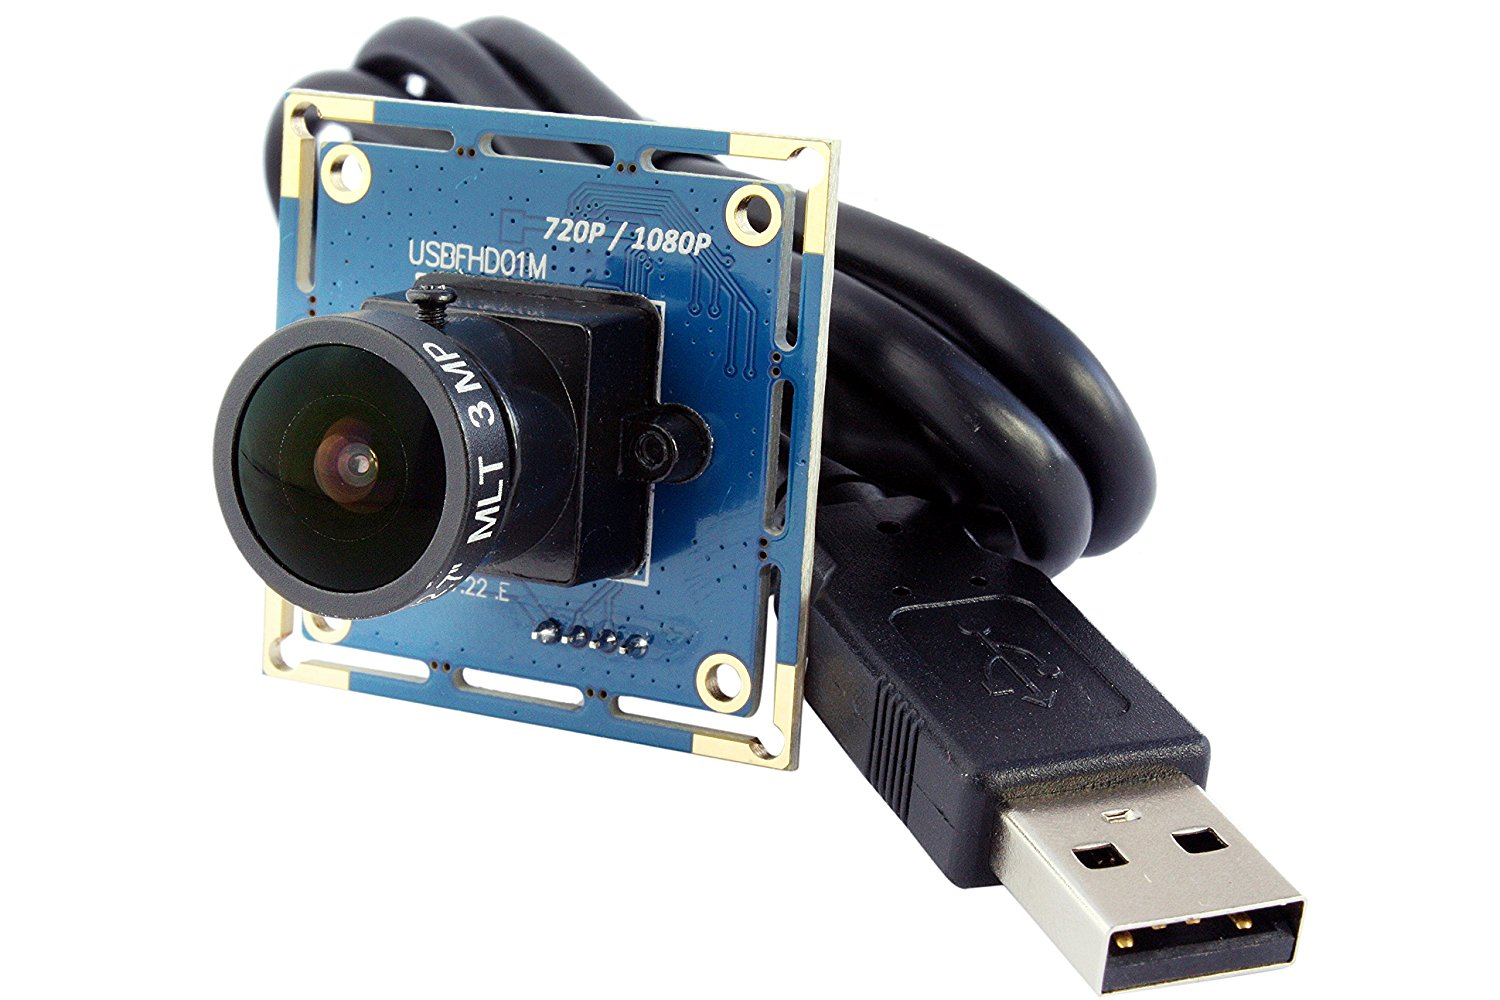
\includegraphics[scale=0.15]{imagenes/robot/camara-usb.jpg}\\
    \caption{Imagen de la cámara USB utilizada.}
  \end{center}
\end{figure}

Los motivos de su elección ha sido principalmente su facilidad de puesta en funcionamiento ya que al tratarse de una cámara USB. Tan sólo debemos conectarla para comenzar con su funcionamiento ya que es detectada 
por prácticamente todas las distribuciones Linux.\\

\subsection{Gamepad}

Gamepad inalámbrico con conexión bluethoot para el manejo del vehículo desde un dispositivo móvil gracias al sistema de acoplamiento del que dispone, Ver figura \ref{figura:control_pad}.

\begin{figure}[H]
  \begin{center}
    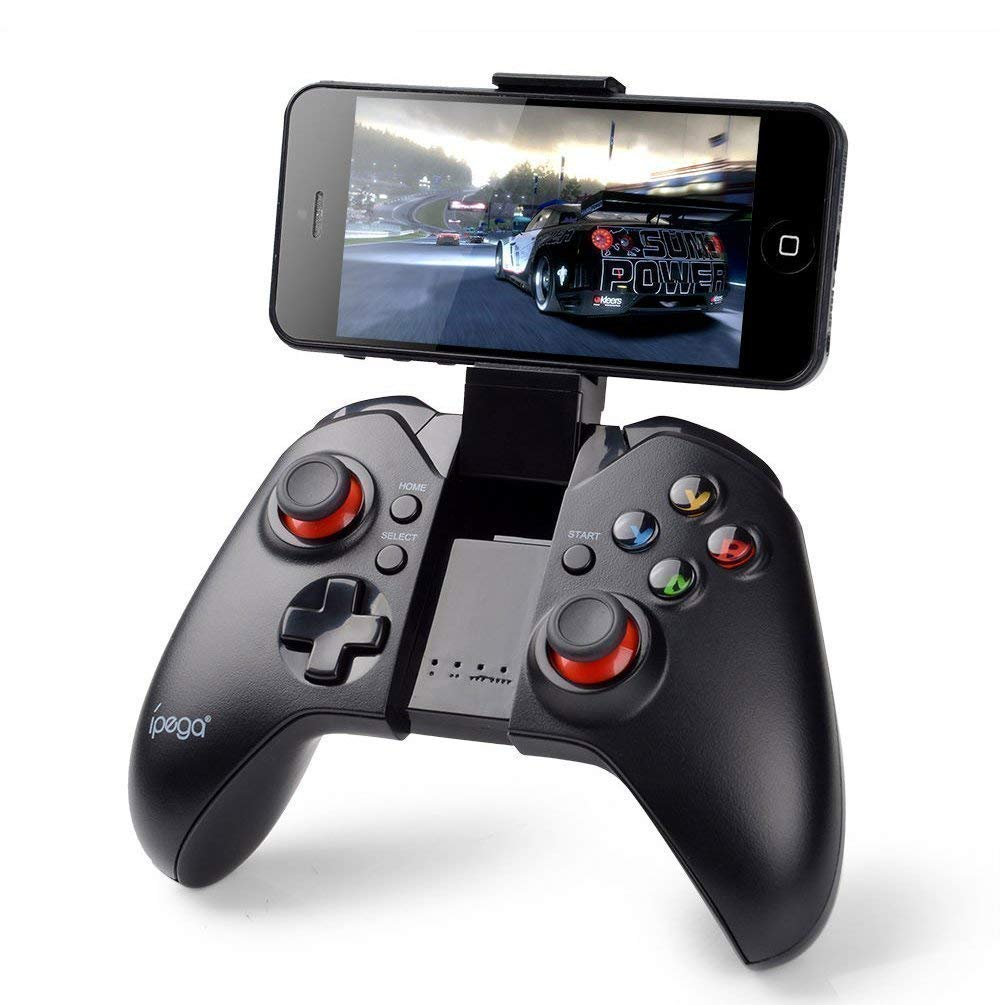
\includegraphics[scale=0.2]{imagenes/robot/control_pad.jpg}
  \end{center}
  \caption{Vista del gamepad utilizado.}
  \label{figura:control_pad}
\end{figure}